% ****** Start of file apssamp.tex ******
%
%   This file is part of the APS files in the REVTeX 4.1 distribution.
%   Version 4.1r of REVTeX, August 2010
%
%   Copyright \textbf{} 2009, 2010 The American Physical Society.
%
%   See the REVTeX 4 README file for restrictions and more information.
%
% TeX'ing this file requires that you have AMS-LaTeX 2.0 installed
% as well as the rest of the prerequisites for REVTeX 4.1
%
% See the REVTeX 4 README file
% It also requires running BibTeX. The commands are as follows:
%
%  1)  latex apssamp.tex
%  2)  bibtex apssamp
%  3)  latex apssamp.tex
%  4)  latex apssamp.tex
%
\documentclass[%
 reprint,
%superscriptaddress,
%groupedaddress,
%unsortedaddress,
%runinaddress,
%frontmatterverbose, 
%preprint,
%showpacs,preprintnumbers,
%nofootinbib,
%nobibnotes,
%bibnotes,
 amsmath,amssymb,
 aps,
%pra,
%prb,
%rmp,
prstab,
%prstper,
floatfix,
%longbibliography
]{revtex4-1}

\usepackage{graphicx}% Include figure files
\usepackage{dcolumn}% Align table columns on decimal point
\usepackage{bm}% bold math
\usepackage{lipsum}
\usepackage{verbatim}
\usepackage{color}
%\usepackage{hyperref}% add hypertext capabilities
%\usepackage[mathlines]{lineno}% Enable numbering of text and display math
%\linenumbers\relax % Commence numbering lines

%\usepackage[showframe,%Uncomment any one of the following lines to test 
%%scale=0.7, marginratio={1:1, 2:3}, ignoreall,% default settings
%%text={7in,10in},centering,
%%margin=1.5in,
%%total={6.5in,8.75in}, top=1.2in, left=0.9in, includefoot,
%%height=10in,a5paper,hmargin={3cm,0.8in},
%]{geometry}

\begin{document}

%\preprint{APS/123-QED}

\title{Reconfigurable Photonic Circuit for Control of Dielectric Laser Accelerators}

\author{Tyler W. Hughes}
\author{Momchil Minkov}%
\author{Shanhui Fan}%
 \email{shanhui@stanford.edu}
\affiliation{Ginzton Laboratory, Stanford University, Stanford, CA, 94305.}

\collaboration{ACHIP Collaboration}
\noaffiliation

\date{\today}

\begin{abstract}
\textcolor{blue}{Dielectric laser acceleration (DLA) is a promising candidate for the next generation of particle accelerators, which makes use of advances in precision nanofabrication, high powered ultrafast lasers, and integrated optics \cite{peralta_demonstration_2013,breuer_laser-based_2013,breuer_dielectric_2014,leedle_dielectric_2015,leedle_laser_2015,wootton_demonstration_2016}.  In DLA, infrared lasers are used to power optical-scale lithographically fabricated dielectric structures, which are designed to create an electromagnetic field pattern that provides extended energy gain to charged particles that traverse the device \cite{plettner_proposed_2006,hughes_method_2017}.  DLA offers orders of magnitude increases in the achievable energy gain per length, or `acceleration gradient', mainly because of the high damage thresholds of dielectric materials when compared to the metal used in conventional RF accelerators \cite{soong_laser_2013}.  The ability to construct compact, inexpensive, and powerful particle accelerators would have numerous applications \cite{england_dielectric_2014,wootton_dielectric_2016}, especially if the technology may be implemented on a chip using an integrated photonic circuit \cite{hughes_-chip_2017}.}
 
\end{abstract}

\maketitle

\section{\label{sec:intro}Introduction}

% intro to DLA
Dielectric laser acceleration (DLA) is a promising candidate for the next generation of particle accelerators, which makes use of advances in precision nanofabrication, high power lasers, and integrated optics \cite{peralta_demonstration_2013,breuer_laser-based_2013,breuer_dielectric_2014,leedle_dielectric_2015,leedle_laser_2015,wootton_demonstration_2016}.  In DLA, infrared lasers are used to power optical-scale lithographically fabricated dielectric structures, which are designed to create an electromagnetic field pattern that provides extended energy gain to charged particles that traverse the device \cite{plettner_proposed_2006, hughes_method_2017}.  DLA offers orders of magnitude increases in the achievable energy gain per length, or `acceleration gradient', mainly because of the high damage thresholds of dielectric materials when compared to the metal used in conventional RF accelerators \cite{soong_laser_2013}.  The ability to construct compact, inexpensive, and powerful particle accelerators would have numerous applications \cite{england_dielectric_2014,wootton_dielectric_2016,wootton_towards_2017}, especially if the technology may be implemented on a chip using an integrated photonic circuit \cite{hughes_-chip_2017}.

% DLA needs to scale to be useful => use integrated optics and reconfigurable / tunable control
A major challenge of DLA is increasing the length of interaction between the driving laser and the electron beam, which is limited by both the beam dynamics and the laser delivery system.  Without an acceleration length at or above the milimeter scale, energy gains from DLA will remain below $1$ MeV, which is not enough for practical applications.  A promising approach to scaling the interaction length involves the use of integrated optics platforms, built with precise nanofabrication, to provide controlled laser power delivery to the DLA.  This scheme would eliminate many free-space optical components, which are bulky, expensive, and sensitive to alignment.  Furthermore, as de-phasing between the electron beam and the driving laser is a large barrier to long interaction lengths, an integrated laser delivery and control mechanism would mitigate this issue by allowing automatic, reconfigurable control over the accelerator structure, similar to what is commonplace in modern RF accelerators.

% We have a system that does this, but it has issues.  (power concentration, fixed powers in each output)
A system for accomplishing integrated optical power delivery was recently proposed in Ref. \cite{hughes_method_2017} in which the laser beam is first coupled into a single dielectric waveguide and then split into several waveguides that spread to power the length of the accelerator structure.  Here, waveguide bends are designed to implement an on-chip `pulse-front tilt', which delays the laser pulses in each waveguide to arrive at the accelerator structure at the same time as the moving electron beam \cite{cesar_optical_2018}.  However, this design has two serious limitations.  First, the design relies on an input facet coupling the laser beam initially to a single waveguide before splitting.  This leads to considerable optical power concentration in the device, which creates a bottleneck for optical damage and nonlinearities.  This limits the maximum power that can be supplied to the device and, in turn, the energy gain of the accelerator.  Secondly, while the phase of each output pulse be tuned using integrated optical phase shifters, the power distribution of the output waveguides is fixed by the fabrication of the splits and bends in the structure and may not be easily tuned later if there are errors.

% the solution is to use direct coupling and some kind of power distribution system
Therefore, an ideal laser coupling scheme for DLA would involve a `one-to-many' coupling scheme that directly couples a single laser pulse into several waveguides.  This would greatly ease the input power limitations present in the power-splitting proposal of Ref. \cite{hughes_method_2017} by reducing the optical damage and nonlinearity bottleneck of the input coupler.  While `one-to-many' coupling techniques exist in the form of grating coupler arrays or combined grating coupler and splitter devices, a tunable $\textit{power}$ distribution system would also be necessary to mitigate the variations in input coupling efficiencies created by such a scheme.  Furthermore, in conjunction with optical phase control and long-range beam-focusing [uwe], a reconfigurable power distribution mechanism will be an essential component for scaling DLA from proof-of principle length scales of 100's of $\mu$m to the scale of modern accelerators.

% we provide a way to do this using MZI meshes
In this work, we propose an integrated power distribution system and corresponding sequential protocol for accomplishing automated, on-chip phase and power control for DLA. For this, we utilize a mesh of integrated Mach-Zehnder interferometers (MZIs), a device that allows for arbitrary unitary operations on-chip \cite{miller_self-configuring_2013,miller_perfect_2015}.  MZI meshes are becoming a fundamental component in integrated, re-configurable optics for mode sorting \cite{miller_sorting_2015,annoni_unscrambling_2017,miller_setting_2017,miller_self-configuring_2018}, quantum information processing \cite{harris_quantum_2017,metcalf_multiphoton_2013,aspuru-guzik_photonic_2012,obrien_photonic_2009}, and optical machine learning hardware \cite{shen_deep_2017, hughes_2018_training}. 

% significance of the work
In this work, we explore the novel application of these reconfigurable optics systems to high power pulse delivery and control for accelerators on a chip, which brings its own interesting set of constraints and challenges.  In conjunction with Ref. \cite{hughes_-chip_2017}, this study gives a roadmap for transitioning the control of DLA systems away from hand-tuned, free-space optical setups to precise, automatically configured integrated optical components.  As such, provides the opportunity to dramatically scale the acceleration length and energy gains of DLA, which is of crucial importance in realizing the exciting applications of these miniature accelerators.

The paper is organized as follows: In Section \ref{sec:system}, we give a systems-level overview of the proposed laser coupling system.  In this Section, we introduce the MZI mesh as a power distribution component for DLA.  In section \ref{sec:algo} we provide a sequential protocol for optimizing the mesh for delivery to the accelerator, which involves layer-wise tuning of individual MZIs using photodetector measurements.  In section \ref{sec:demo}, we perform numerical simulations of reconfiguring such a mesh to demonstrate our method. Then, in Section \ref{sec:discussion}, we discuss the scalability of our approach and other considerations before concluding in Section \ref{sec:conclusion}.

\section{\label{sec:system}Reconfigurable control system}

\begin{figure}
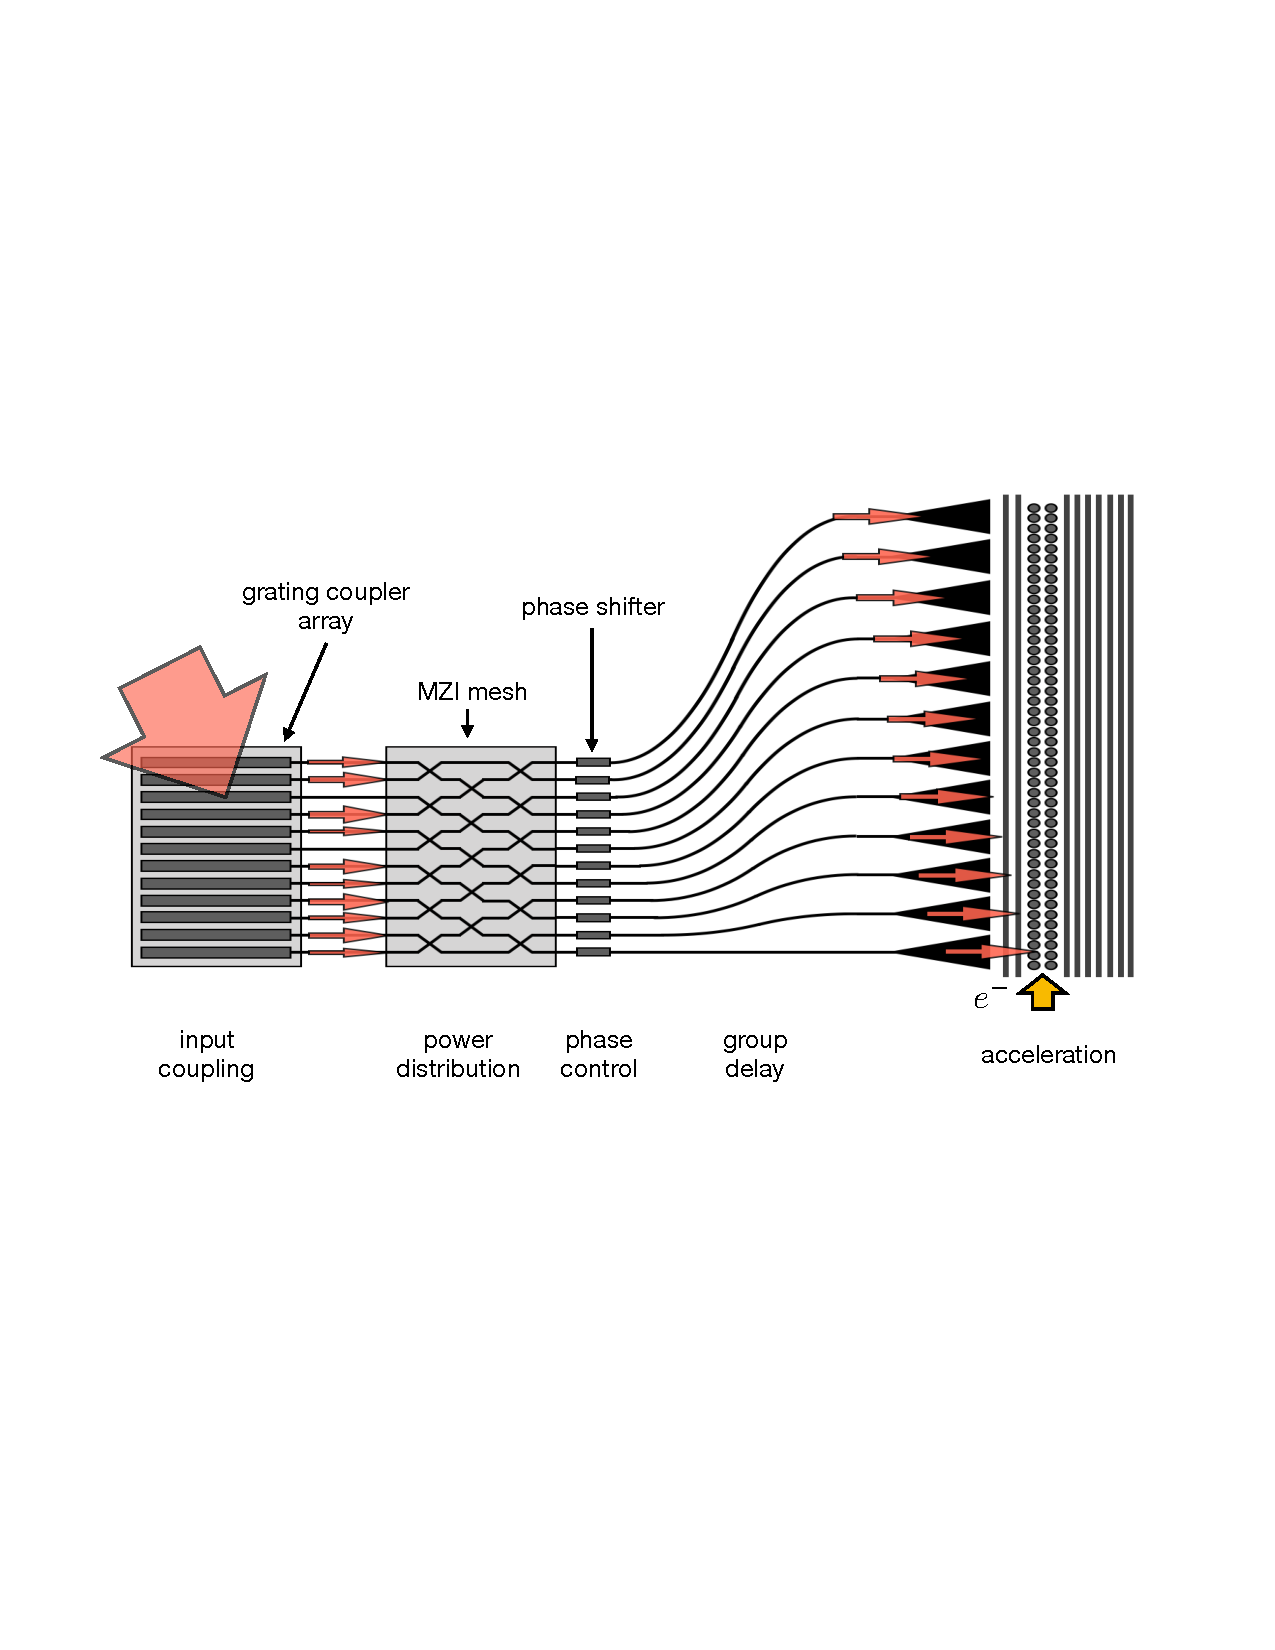
\includegraphics[width=\columnwidth]{Fig1.pdf}
\caption{\label{fig:setup} \textbf{Schematic of the proposed DLA laser delivery control system.} An input pulse (large red arrow) is focused to an array of grating couplers on the surface of the chip.  The pulse is directly coupled into several waveguides, likely with random phase and power distribution.  To mitigate this issue, the waveguides next enter a mesh of MZIs, which is sequentialally adjusted, using the protocol from this paper, to provide uniform output powers.  A layer of optical phase shifters is applied to each waveguide to ensure that the pulses are in phase once they reach the accelerator gap.  Lithographically-defined bends then spread the waveguides such that they power a longer length of acceleration.  These bends are also designed to provide a group delay to the pulses such that they reach the accelerator as the same time as a moving electron bunch.  Finally, the waveguides are tapered and are coupled into the accelerator structure, where they will provide energy gain to the electron beam.}
\end{figure}

Here we will give an overview of the proposed reconfigurable laser coupling scheme for DLA.  A schematic of our system is shown in Fig. \ref{fig:setup}. The input coupling, power distribution, phase control, group delay, and DLA coupling stages are performed sequentially.

In our design, the driving laser pulse is first focused onto an input element that directly splits the optical power into several waveguides.  As mentioned, this coupling strategy eliminates the optical damage and nonlinearity bottleneck and therefore greatly improves the power that can be safely supplied by the driving laser. This element could take the form of a grating coupler array [cite array] or combined grating coupler and power splitter geometry [cite Neil's link].  Adjoint-based optimization techniques [neils grating couplers] may be employed to design novel input coupling components with improved coupling efficiency, less variation between powers, or significantly more output waveguides, although this is outside the focus of this work.

\begin{figure}
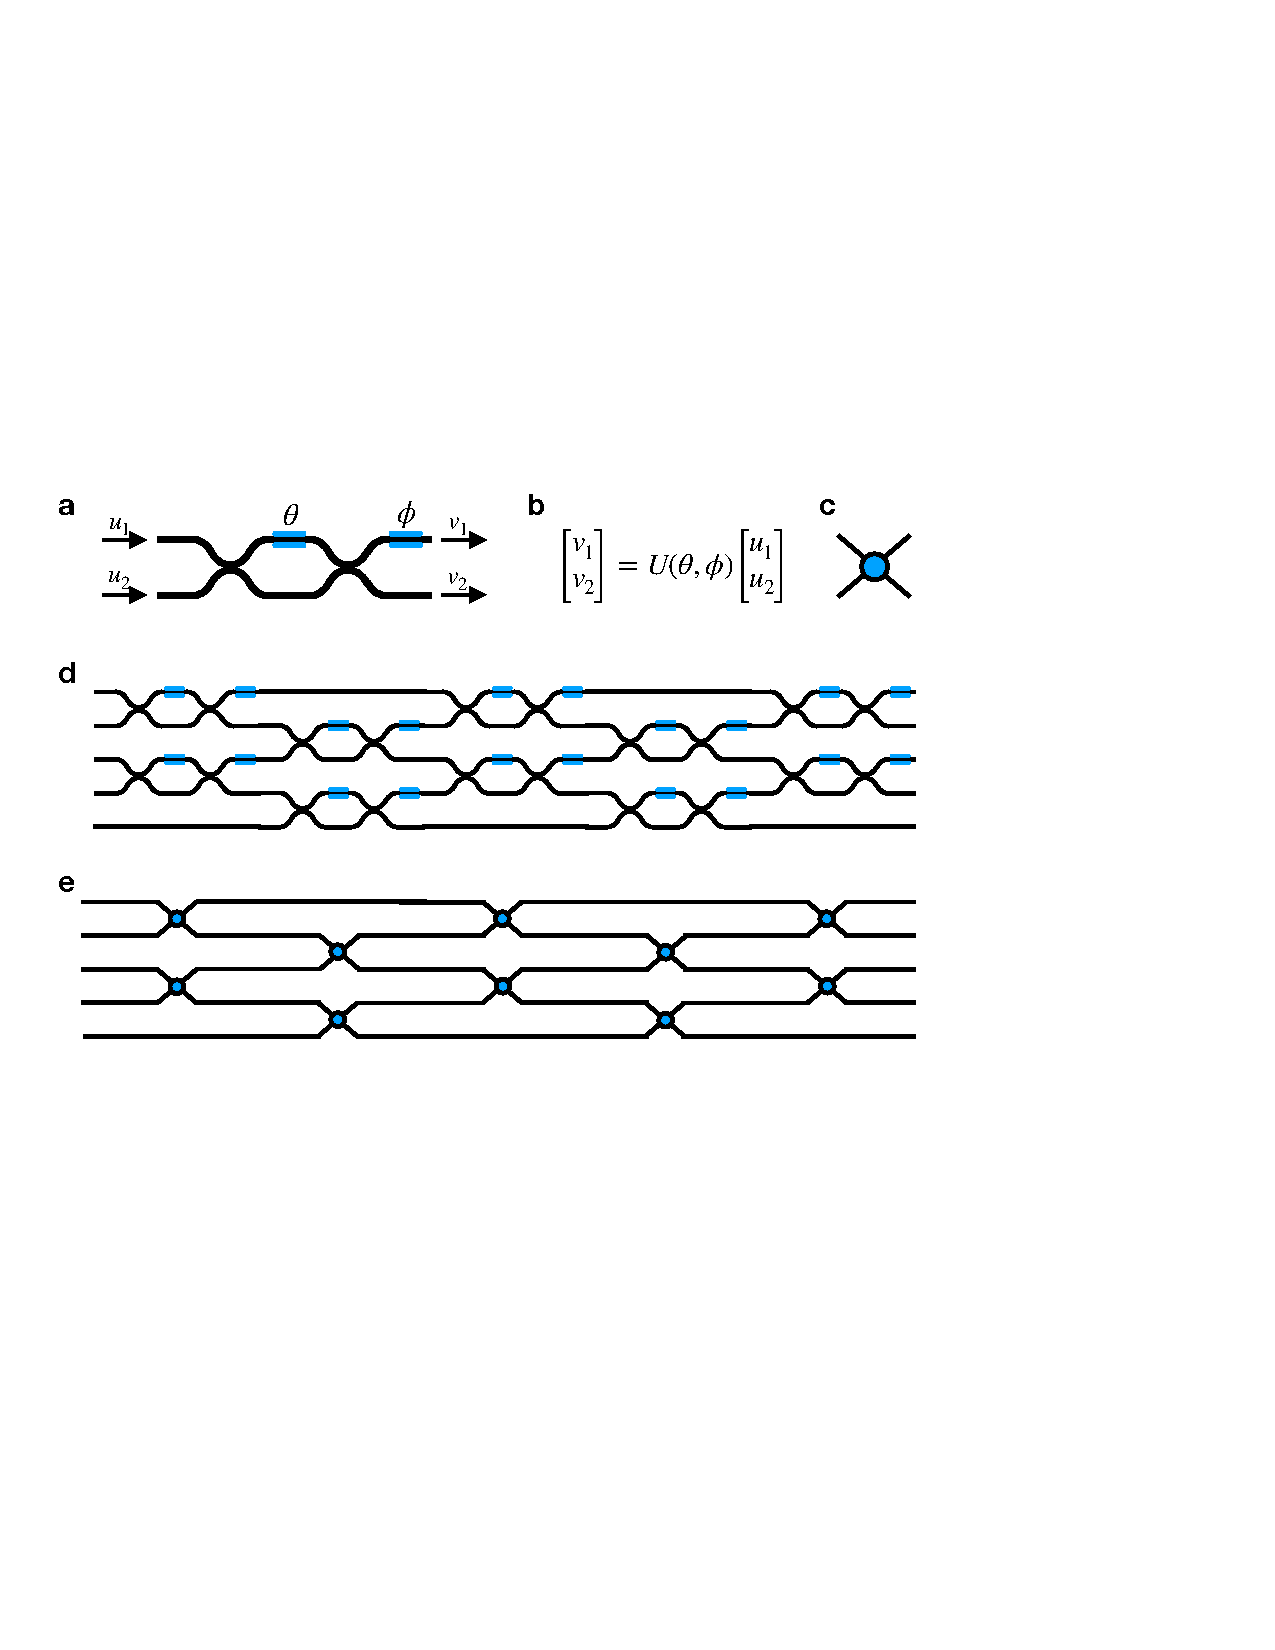
\includegraphics[width=1\columnwidth]{Fig2.pdf}
\caption{\label{fig:mesh} \textbf{Diagram of MZI mesh for power distribution.} \textbf{a}, Diagram of a single MZI consisting of two input ports and two output ports.  Where the two arms come together, a 50-50 beam-splitter operation is performed.  The blue regions indicate tunable optical phase shifters with added phases marked as $\theta$ and $\phi$.  \textbf{b}, The MZI represents a tunable unitary transformation on its inputs $[u_1, u_2]^T$ to give outputs $[v_1, v_2]^T$.  \textbf{c}, Simplified diagram representing an MZI in the following figures.  One may think of this element as a tunable power switch. \textbf{d}, Individual MZIs are combined into meshes, which may implement tunable unitary operations on several inputs.  Shown is a 'Clements' Mesh geometry, which was used in this work. \textbf{e}, Schematic of the Clements mesh in \textbf{d} using the simple MZI diagram in \textbf{c}.}
\end{figure}

After coupling, due to fabrication and alignment errors, there will be much variation in the power distribution of each waveguide. To ensure that an equal amount of power is supplied to the accelerator, we introduce a power distribution component that is comprised of a mesh of MZIs.  As diagrammed in Fig. \ref{fig:mesh} \textbf{a}-\textbf{c}, each individual MZI is comprised of two beam-splitters and two optical phase shifters, $\theta$ and $\phi$, which can be electrically adjusted to perform the following unitary operation on its two inputs \cite{reck_experimental_1994,clements_optimal_2016,shen_deep_2017}
\begin{align}
\begin{split}
    \begin{bmatrix}
      v_1 \\ v_2
    \end{bmatrix}
    =&~U(\theta, \phi) 
    \begin{bmatrix}
      u_1 \\ u_2
    \end{bmatrix}
    \\
    =&~e^{i\frac{\theta}{2}} e^{i\frac{\phi}{2}}
    \begin{bmatrix}
      e^{i\frac{\phi}{2}}\cos{\frac{\theta}{2}} &
      e^{i\frac{\phi}{2}}\sin{\frac{\theta}{2}} \\
      e^{-i\frac{\phi}{2}}\sin{\frac{\theta}{2}} & 
      e^{-i\frac{\phi}{2}}\cos{\frac{\theta}{2}}
    \end{bmatrix}
    \begin{bmatrix}
      u_1 \\ u_2
    \end{bmatrix}.
\end{split}
\end{align}
%

As in Fig. \ref{fig:mesh} \textbf{d},\textbf{e}, several MZIs may be combined in a mesh, which is capable of performing unitary operations over an arbitrary large number of inputs.  There are several possible configurations of the MZI mesh, each with their own benefits and drawbacks.  In this application, the mesh must be compact enough to fit on the chip and also have a bandwidth large enough to handle sub-ps pulses.  Whereas many meshes are capable of performing arbitrary unitary operations, for this power delivery problem it is only necessary to sort random inputs into uniform outputs.  With these considerations in mind, the `Clements' mesh geometry \cite{clements_optimal_2016} is best suited for this application.   As diagrammed in Fig. \ref{fig:mesh} \textbf{d},\textbf{e}, the Clements mesh requires fewer layers than other designs \cite{reck_experimental_1994} and also is more robust to optical losses because of its symmetric layout.  Furthermore, it may be implemented in a `shallow` mesh with fewer layers than input ports.  This is especially useful for DLA power distribution problem as we will show that only a few layers are required for adequate power equalization.  %more details in supplementary?

In the following Section we describe a sequential protocol for optimizing the Clements mesh for power distribution. As our protocol uses local information about the power within the network, we require the inclusion of integrated optical photodetectors, such as those used in [].  Alternatively, an imaging system, in conjunction with scattering elements, may be used to read this information from above the chip.

Once the power in each waveguide is equalized, we must correct the phase of each laser pulse such that it is synchronous with the electron beam. While the phase shifters may be adjusted to maximize energy gain, they may also be used to incorporate other functionality, such as beam focusing, total beam transmission, deflection, or diagnostics.  Beam energy measurements, performed periodically along the accelerator, may be used as a signal to automatically configure the optical phase shifters.

% \subsection{group delay}
Once the power and phase are sufficiently controlled, we must delay the laser pulse in each waveguide so that it arrives at the accelerator gap the same time as the moving electron beam. To do this, we introduce lithographically-defined bends in the waveguides to provide a delay that is matched to the electron arrival, producing of the integrated optics analogue of a pulse-front tilt \cite{cesar_optical_2018}. The mathematical details of the bend design are described in the supplementary material of Ref. \cite{hughes_-chip_2017}.

% \subsection{DLA coupling}
The final stage involves coupling the waveguide mode into the acceleration channel.  Ideally, an inverse taper may be placed at the end of each waveguide to spread the mode area to match the geometry of the electron beam.  Then, an accelerator structure may be placed adjacent to the end of the waveguides.  Alternatively, the accelerator structures and tapers may be part of the same system and may be designed following ideas from proposed buried grating structures \cite{chang_silicon_2014}, or using inverse design techniques, such as what was shown Ref. \cite{hughes_method_2017} for free-space coupling.  Dielectric mirrors may be used to design the resonance of the acceleration cavity and provide back reflection if a single-sided drive is used (as pictured in Fig. \ref{fig:setup}).  While Ref. \cite{hughes_-chip_2017} argued that a moderately resonant acceleration cavity with quality factor of several hundred would be necessary to lower the input power to mitigate the input facet bottleneck introduced by that design.  In this proposal, because that bottleneck is eliminated, a less resonant structure may be used.

\section{\label{sec:algo}Power Distribution Protocol}

Here we describe a power distribution protocol on a Clements mesh that is optimal for equalizing the power coming from a random input source.  The goal of power equalization is to find the settings of each of the integrated phase shifters such that, given an input to the mesh, there is an equal power in each output port.  A naive implementation of this may involve performing a global optimization over each of the phase shifters.  However, when the number of degrees of freedom increases (for example, for a very large accelerator), this becomes unfeasible as the time to solve scales exponentially with the number of MZIs. Fortunately, the protocol presented in this work has that property that each MZI may be tuned individually and in sequence, layer by layer, from input to output. If there are $N$ MZIs, then our method involves sequentially solving $N$ optimization problems with 2 degrees of freedom.  In contrast with the exponential scaling of the full optimization problem, here, the amount of time to solve the system scales linearly with the number of MZIs.

\begin{figure}[!ht]
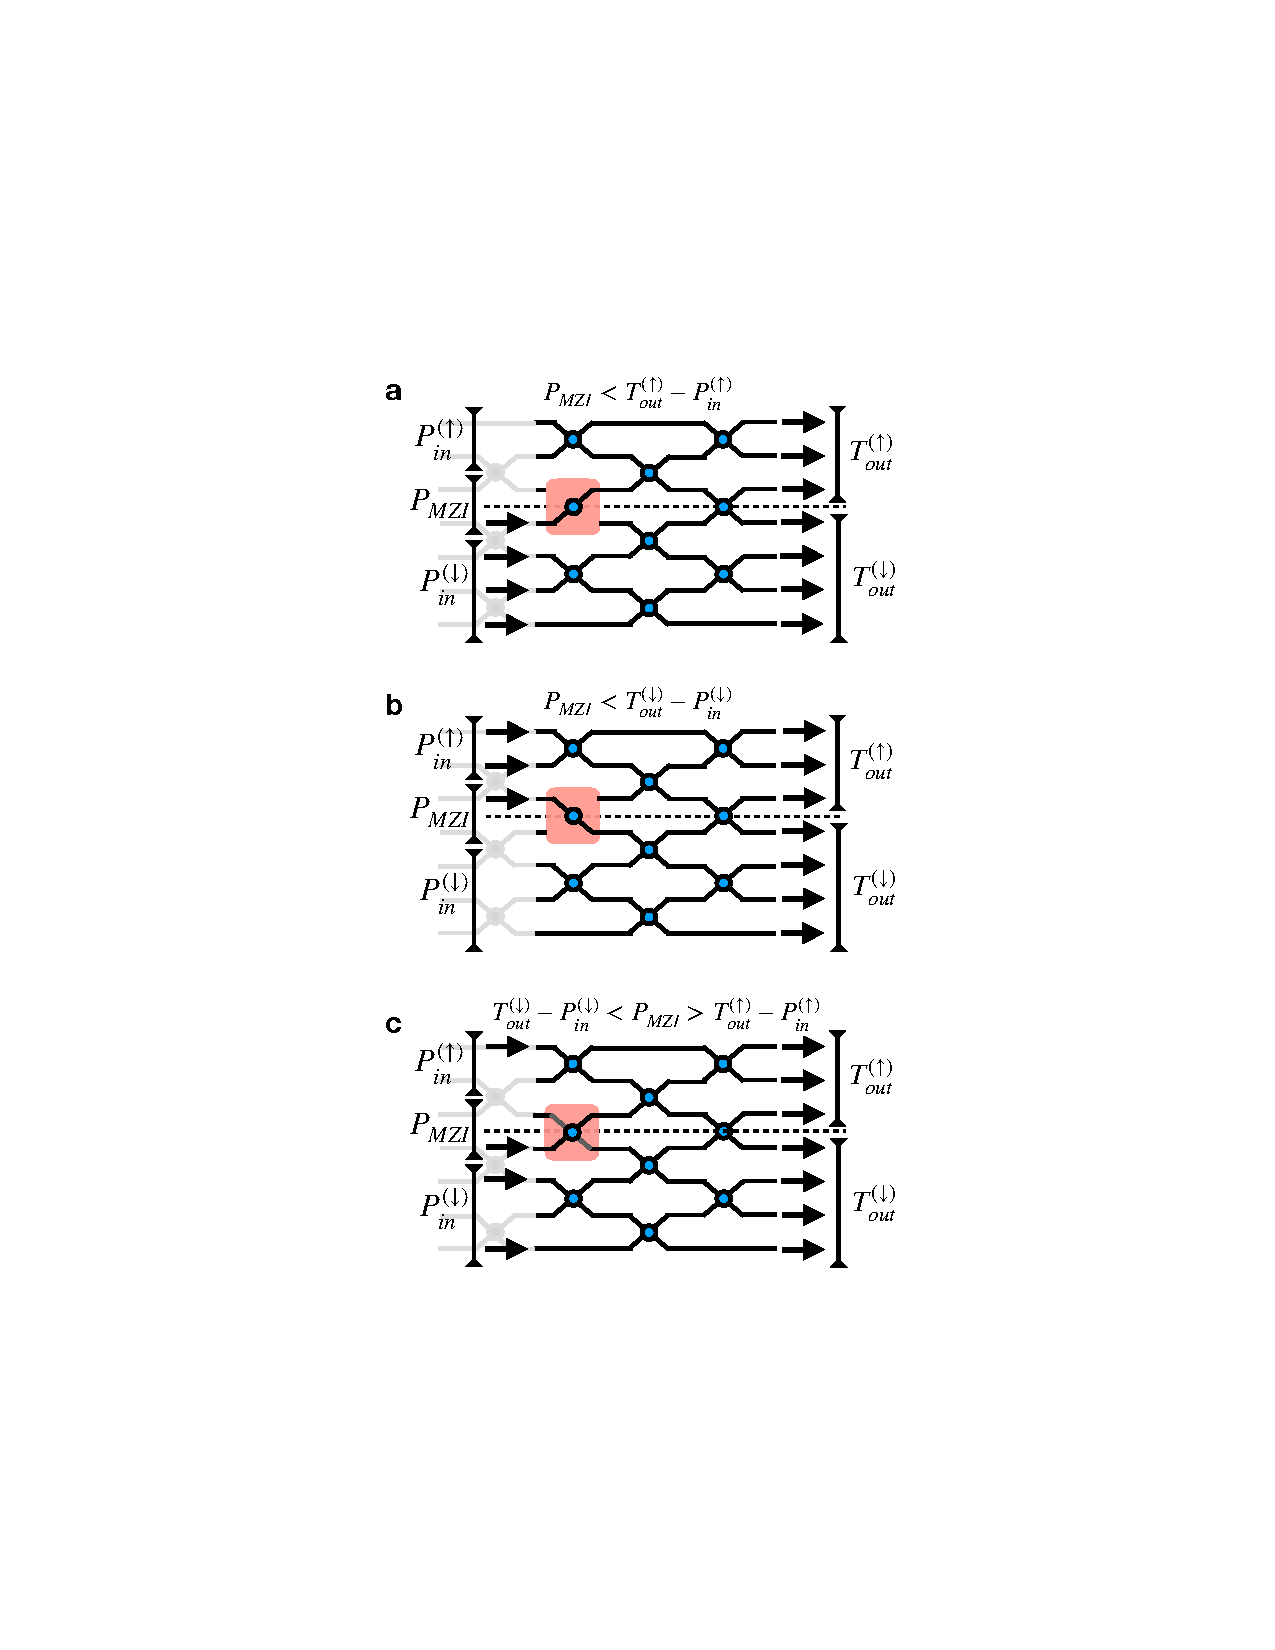
\includegraphics[width=0.7\columnwidth]{Fig3.pdf}
\caption{\label{fig:algo} \textbf{Sequential algorithm for tuning single MZI.} The red square outlines the MZI being tuned.  Black arrows on the left indicate input power to the current layer, black arrows on the right indicate desired output powers (uniform in this case).  The dotted line separates the mesh into powers above and below the MZI.  \textbf{a} When there is more power needed in the ports above the MZI than are supplied in the ports leading into the MZI and above, the MZI should output all of its power to its top output port. \textbf{b} When there is more power needed in the ports below the MZI than are supplied in the ports leading into the MZI and below, the MZI should send all of its power to the bottom output port.  \textbf{c} In the intermediate case, the MZI should output just enough power to its top and bottom output ports to match the target power requirements.}
\end{figure}

Our protocol is diagrammed in Fig. \ref{fig:algo}, in which we show how to tune a single MZI (red) in a given layer of the network based purely on information about the powers coming into that layer.  For generality, we assume that we wish to tune this mesh to achieve an arbitrary target output power distribution $T_{out}^{(i)}$ for each of the ports $i \in \{1..N\}$.  We also assume that we have knowledge of the power at each of the ports, $i$, coming into this layer, labelled $P_{in}^{(i)}$.

The essential idea of the protocol is to tune each MZI to direct power to either its top port or its bottom port, depending on where power is deficient in the input to this layer and where it is needed in the final output target. To visually represent this idea, in Fig. \ref{fig:algo}, we show a horizontal line bisecting the mesh through the MZI in question and now define some terms for concreteness.  Assuming that the MZI is located vertically within the mesh with its top input  port at index $j$, defining top port index $j=1$ and bottom port index $j=N$, we may define the sum of power input to this specific MZI as
\begin{equation}
    P_{MZI} \equiv P_{in}^{(j)} + P_{in}^{(j+1)}.
\end{equation}
The sum of the powers input to this layer both above and below this MZI, respectively, are defined as
\begin{align}
    P_{in}^{(\uparrow)} &\equiv \sum_{i=1}^{j-1} = P_{in}^{(i)} \\
    P_{in}^{(\downarrow)} &\equiv \sum_{i=j+2}^N = P_{in}^{(i)}.
\end{align}
Finally, the target powers above and below this MZI, respectively, are defined as
\begin{align}
    T_{out}^{(\uparrow)} &\equiv \sum_{i=1}^j = T_{out}^{(i)} \\
    T_{out}^{(\downarrow)} &\equiv \sum_{i=j+1}^N = T_{out}^{(i)}.
\end{align}

Now, using these values, we give a prescription for directing the power out of the MZI to optimally match the target.  We notice that there are three distinct regimes to consider.  These are each diagrammed separately in the subplots of Fig. \ref{fig:algo}.  

A simple case is when the sum of power supplied to the MZI and the ports \textit{above} it is less than the sum of power needed at the final output \textit{above} the MZI.  This is also written as
\begin{equation}
    P_{MZI} < T_{out}^{(\uparrow)} -  P_{in}^{(\uparrow)}.
\end{equation}
In this case, the optimal strategy for the MZI is to direct all of its power to the \textit{top} output port, as shown in the red box of Fig. \ref{fig:algo} \textbf{a}.

The opposite case is when the sum of power supplied to the MZI and the ports \textit{below} it is less than the sum of power needed at the final output \textit{below} the MZI.  This is also written as
\begin{equation}
    P_{MZI} < T_{out}^{(\downarrow)} - P_{in}^{(\downarrow)}.
\end{equation}
Conversely, in this case, the optimal strategy for the MZI is to direct all of its power to the \textit{bottom} output port, as shown in the red box of Fig. \ref{fig:algo} \textbf{b}.

The middle case is where the power in the MZI is enough to cover the deficiencies in both the top and the bottom sections of the mesh.  This can be written as
\begin{align}
\begin{split}
    P_{MZI} &> T_{out}^{(\uparrow)} -  P_{in}^{(\uparrow)} \\
    P_{MZI} &> T_{out}^{(\downarrow)} - P_{in}^{(\downarrow)}.
\end{split}
\end{align}
In this case, the MZI need only supply $T_{out}^{(\uparrow)} - P_{in}^{(\uparrow)}$ of its power to the top port.  The leftover power may be transmitted to the down port, which, by power conservation, will be equal to $T_{out}^{(\downarrow)} - P_{in}^{(\downarrow)}$ if the target powers are normalized such that $\sum_{i=1}^{N}P_{in}^{(i)} = \sum_{i=1}^{N}T_{out}^{(i)}$.  This is demonstrated in Fig \ref{fig:algo} \textbf{c} where the MZI performs a partial splitting of power.

With this protocol, one may thus optimize each MZI sequentially through the mesh.  To do this optimally, the MZIs must be tuned layer-by-layer from input to output.  Within each layer, a set of integrated photodetectors must be used to measure $P_{in}^{(i)}$ for all ports $i$.  Then, the individual MZIs in this layer may be tuned in parallel or in any order desired.

\section{\label{sec:demo}Numerical Demonstration}

\begin{figure}
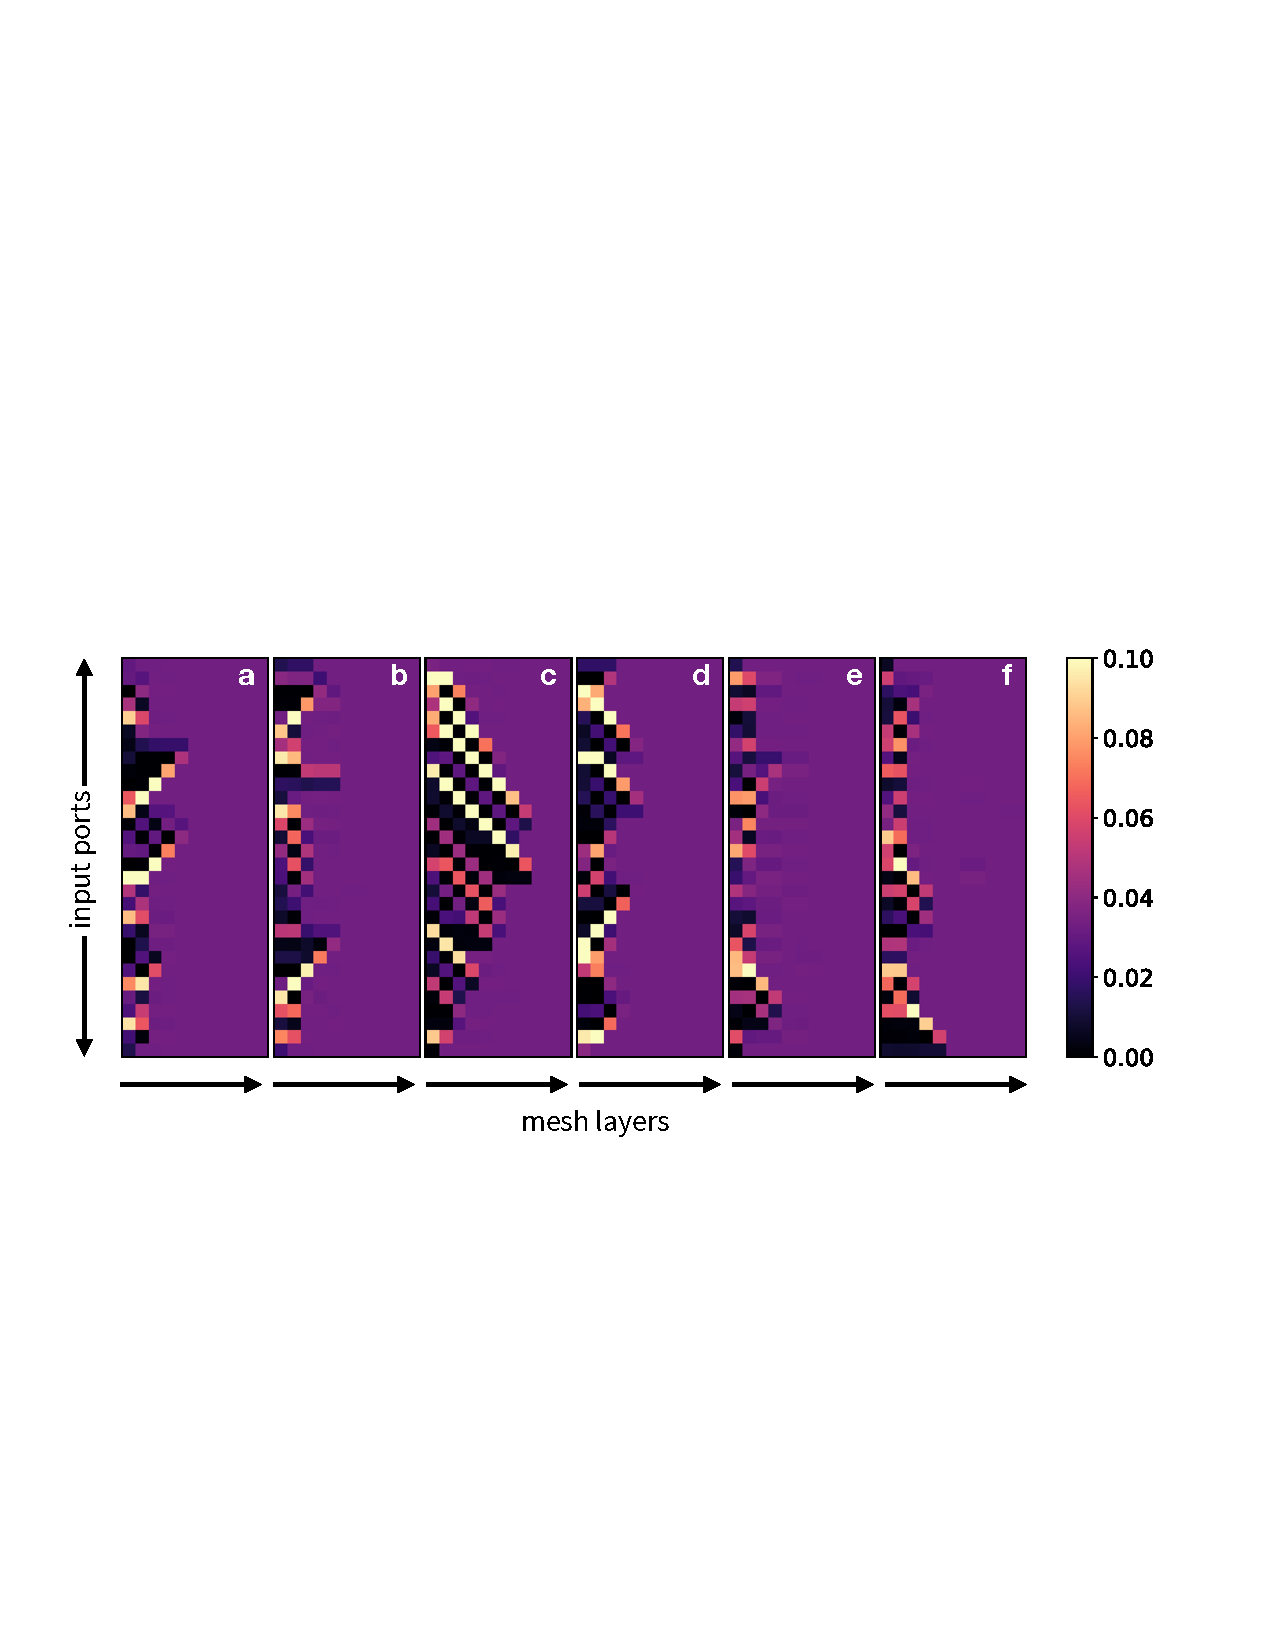
\includegraphics[width=1\columnwidth]{Fig4.pdf}
\caption{\label{fig:equalization} \textbf{Demonstration of mesh optimization for equal power distribution.} \textbf{a}-\textbf{f} The powers in each port after optimizing the mesh for uniform output power given several random input powers.  The vertical axis represents the input port and the horizontal axis represents the layer.  Power flows from left to right.  Equalization is achieved, on average, after only around 5 layers given this network with 30 ports.}
\end{figure}

To demonstrate our protocol, we perform numerical simulations of a Clements mesh and optimize it for power equalization from random inputs to uniform outputs. A software package [] was written to simulate the mesh and perform the optimizations. This package was written such that it may eventually be augmented to interface with a physical MZI mesh to act as a control mechanism.  The result of 6 runs is shown in Fig \ref{fig:equalization}, in which we plot the power in each port within the network after it is optimized using this procedure.

For each run, we initialize a Clements mesh with $N = 30$ input ports and $M = 10$ layers.  Then, we generate a vector of random input powers to couple to the mesh, $P_{in}$.  When constructing $P_{in}$, each element is chosen uniformly at random between 0 and 1 and then the whole vector is normalized such that it sums to 1.  For demonstration purposes, we optimize the mesh to output to a uniform output target $T_{out}$, where each element of $T_{out}$ is equal to $1/N$, such that both the input and target powers are normalized to each sum to 1.  Although a uniform output target was chosen as it is most applicable to DLA applications, the same protocol may be equally applied to other targets with similar results.

We then step through the mesh from input to output, tuning all MZI's in a given layer according to the protocol introduced in the previous section before moving to the next layer.  To perform the tuning, we use a simple downhill simplex algorithm [cite?] to tune the phase shifters ($\theta$ and $\phi$) in the MZI until they output the correct power as described by the protocol.  From Fig. \ref{fig:equalization}, we notice that equalization is acheived after only around 5 layers on average.

To understand how the device operation scales with the number of layers, we studied the performance of the equalization routine as the number of ports are increased.  The results are shown in Fig. \ref{fig:scaling} where we show the mean-squared-error between the power in each layer, defined as 
\begin{equation}
    MSE = \frac{1}{2}\sum_{i=1}^N \left( P_{in}^{(i)} - T_{out}^{(i)} \right)^2.
\end{equation}
We then sweep through different mesh sizes and average the data for each mesh over 5 runs with different random inputs.  The number of layers needed for equalization grows slowly as the network size is increased.  This suggests that for very large networks (with > 100-1000 ports), only several tens of layers of MZIs may be needed in the Clements mesh to perform power equalization.

\begin{figure}
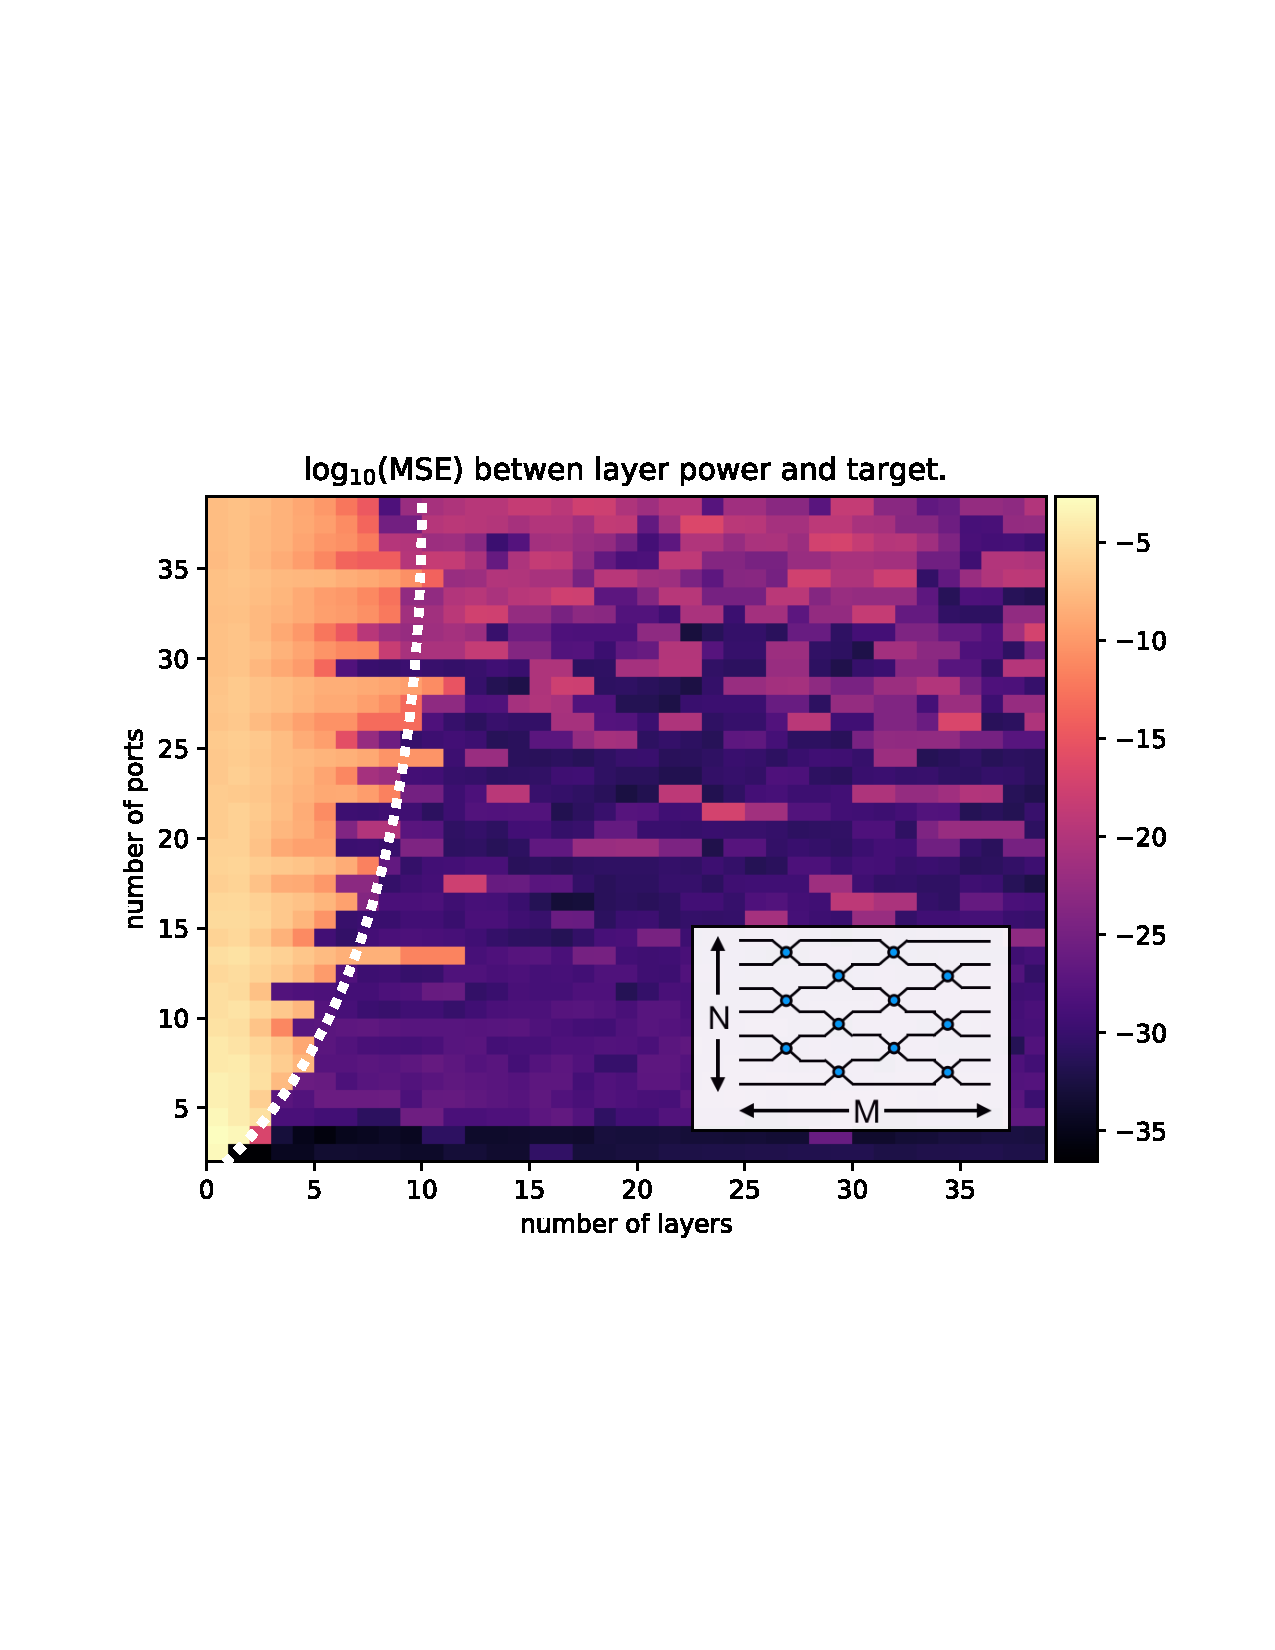
\includegraphics[width=1\columnwidth]{Fig5.pdf}
\caption{\label{fig:scaling} \textbf{Analysis of mesh performance vs. number of input ports}.  We plot the mean-squared-error of the power in each layer with the target power}
\end{figure}

\section{\label{sec:discussion}Discussion}

Our proposal provides a method for automated control of DLA systems and eliminates the major issues with previous laser coupling schemes.  We show that MZI meshes are a promising candidate for a power distribution system for DLA systems our findings may be applied to other applications for integrated optical power routing.  The proposal given here only uses existing optical components and, therefore, should be feasible for an experimental demonstration.

The novel procedure we introduce for optimizing the MZI mesh to achieve arbitrary power distribution is highly efficient in terms of number of measurements and phase shifter tunings.  For a mesh with $N$ ports and $M$ layers, our protocol replaces one large optimization problem with $2NM$ degrees of freedom to $MN$ independent optimization problems with 2 degrees of freedom each.  This improves the feasiblity of implementing this protocol on large meshes with thousands of input ports, for example, which may be needed for large-scale DLA.

We show that a shallow Clements mesh is sufficient for equalizing power from random inputs.  This is of crucial importance for DLA applications where there are limitations on the chip space available for phase shifters and electrical contacts.  It also means that a shorter propagation length within the waveguides can be achieved, which reduces the possible nonlinear effects.  Having a shallow mesh also allows the device to retain a large bandwidth, which decreases with the number of MZIs in an optical path.  This is crucially important for handling sub-picosecond driving pulses used in DLA.  However, the bandwidth of MZI meshes and its scaling with respect to network size is not yet fully understood.  This will need to be tested experimentally or with a separate numerical study.

The optimization protocol presented here decomposes the global optimization problem of tuning the entire mesh into several subproblems involving tuning the invidiual MZIs.  However, alternatively a gradient-based approach may be used to train the full mesh.  It was shown previously \cite{hughes_2018_training} that the gradient of the output of an MZI mesh with respect to the dielectric function of each of the phase shifters may be measured experimentally using adjoint fields []. Interestingly, for the case of maximizing the acceleration of a DLA, it was independently shown that the corresponding adjoint fields are given exactly by the fields radiated by the electron beam \cite{hughes_method_2017}.  This suggests an interesting approach to optimizing the MZI mesh towards maximum acceleration by first measuring the radiation from test electron beam, and then using the protocol from Ref. \cite{hughes_2018_training} to compute the gradient of the acceleration with respect to each of the phase shifters.  With this, one may do parallel, gradient-based updates of the phase shifters and optimize arbitrarily large grids with high efficiency. This idea may be explored in a future study.

\section{\label{sec:conclusion}Conclusion}

This study further shows that integrated optical power delivery systems are worth continuing to pursue for DLA.  Specifically, we show that they give a path towards automatic power distribution, which is an essential component towards scaling DLA to longer length scales and exciting applications.  We also provide a novel application of the MZI mesh, which is already finding many applications in other exciting reconfigurable optics applications.  Our efficient protocol for optimizing an MZI for arbitrary power distribution may find many applications beyond DLA.

Integrated optics, and reconfigurable optics in general, allows unique opportunities for accelerators on a chip to take advantage of high precision control and automatic compensation for errors from fabrication, alignment, or drift. This study presents a promising avenue for accomplishing extended acceleration lengths for these accelerators and eventually may enable future applications of DLA technology.

\bibliography{DLA_Phase_Control}

% \appendix

% \section{\label{appx} Numerical Simulation Model}

% Here we give details on the mathematics of the simulation from Section \ref{sec:demo}.  We show how the power distribution stage is performed on a system with $N$ total input and output ports.  It follows that, without loss or backscattering, the system may be described by a $N \times N$, unitary matrix, `$M$', where $M_{i,j}$ relates the modal amplitude at input port $j$ to the modal amplitude at output port $i$.  

% As there are $2N-3$ MZIs in the system, the matrix $M$ is constructed by successively multiplying $2N-3$ corresponding $N \times N$ matrices correpsonding to each MZI.  With these MZI matrices labelled $M_i$ for $i = 1...2N-3$ from left to right, 
% \begin{equation}
% M = \prod_{i=2N-3}^1 M_i.
% \end{equation}

% Here $M_i$ is matrix with ones along its diagonal and a $2 \times 2$ matrix, $B$, corresponding to the MZI, embedded at an index that corresponds to the $i$-th MZI's position in the network.  For an example, 

% \begin{equation}
% M_1 = 
% \begin{bmatrix}
%   1 & 0      & 0 &        &  0       & 0       \\
%   0 & 1      & 0 & \cdots &  0       & 0       \\
%   0 & 0      & 1 &        &  0       & 0       \\
%     & \vdots &   &        &  0       & 0       \\
%   0 & 0      & 0 &    0   &  B_{1,1} & B_{1,2} \\
%   0 & 0      & 0 &    0   &  B_{2,1} & B_{2,2}
% \end{bmatrix}
% \end{equation}

% Where, $B$ is parameterized by the phase of each of the integrated phase shifters in the MZI, $\phi_1$ and $\phi_2$ as
% \begin{equation}
% B(\phi_1,\phi_2) = -ie^{i\phi_2/2}
% \begin{bmatrix}
%   -\sin(\phi_2/2) & \cos(\phi_2/2)e^{i\phi_1} \\
%   \cos(\phi_2/2) & \sin(\phi_2/2)e^{i\phi_1}
% \end{bmatrix}.
% \end{equation}
\end{document}